\chapter{Validation}

\section{Analytical solution}
To test the FEM solution analytically, a plate of length 1 m and height 1 m is loaded in the x direction with a force of 100 kN. A graphic representation of this problem can be found in the image below.

\begin{figure}[h!]
    \parbox [t]{\textwidth}
        {
        \center
        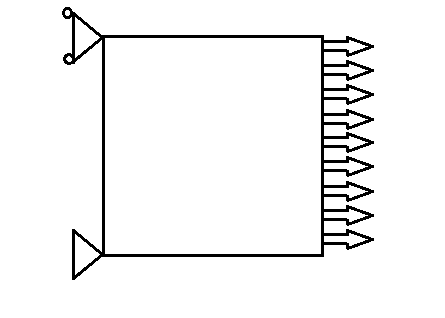
\includegraphics[width=0.5\textwidth]{IMG/analytisch.png}
        }
\end{figure}

This is a thin plate and therefore plane stress can be assumed. In plane stress the following relation holds:
\[\sigma=\varepsilon*E\]
The value of the Young's modulus is 70 GPa. The stress is calculated by dividing the force by the length of the side of the plate. From this a strain of \(1.4286*10^{-6}\) can be found. 
In the FEM the left side of the plate is constrained in the x direction and the force is applied to the right side. The displacement of the right side of the plate due to this force is also \(1.4286*10^{-6}\), exactly the same as the analytical solution. 

\section{Area vs Weight}
Every element in the FEM simulation has a weight factor which is scaled to the size the element has. For the standard triangle the weight factor is $0.5$, but when the standard triangle is fitted over the actual element this value changes. The sum of all the elements should add up to the total area of the material. This does not show that our code is correct, but is does show that the weight factors according to all elements are correct. The mesh of the Multihole has a surface of $82.58$ and the sum of the weights is $82.729$. Assumed is this difference is a consequence of the discrete mesh. The linear elements are not able to follow the arcs of the holes. With a finer mesh the difference should become smaller. To check this the mesh is refined which leads to a sum of weights of $82.6181$ which gives a better representation.
